\documentclass[11pt,a4paper]{article}
\usepackage[russian]{babel}
\usepackage[utf8]{inputenc}
\usepackage{amsmath}
\usepackage{mathtools} 
\usepackage[russian]{babel}
\usepackage{hyperref}
\usepackage{amssymb}
\usepackage{multicol}
\usepackage{bm}
\usepackage[hcentering, bindingoffset = 10mm, right = 15 mm, left = 15 mm, top=20mm, bottom = 20 mm]{geometry}
\newcounter{prim}
\newenvironment{prim}{%
	\addtocounter{prim}{1}
	\noindent{\\
		\textbf{\noindentПример \arabic{prim}\\}}%
}{}

\DeclareMathOperator{\tr}{\mathop{tr}}
\DeclareMathOperator{\Ker}{\mathop{Ker}}
\DeclareMathOperator{\im}{\mathop{Im}}
\DeclareMathOperator{\const}{\mathop{const}}
\DeclareMathOperator{\rg}{\mathop{rg}}
\newtheorem{definition}{Определение}[section]
\newtheorem{theorem}{Теорема}[section]
\renewcommand{\labelenumi}{\asbuk{enumi})}

\begin{document}
	\part*{Лабораторная работа 3.6.1}
	\part*{Спектральный анализ электрических сигналов. Компьютерный вариант}
	\textbf{Работу выполнили:} \\
	{\itshape Морозов Матвей \\ Бабушкина Татьяна \\ 678 группа} \\\\
\textbf{Цель работы:} изучение спектрального состава периодических электрических сигналов.
\\\\
\textbf {В работе используются:} персональный компьютер, USB-осциллограф АКИП-$4107$, функциональный генератор WaveStation $2012$, соединительные кабели.
\\
\\
\part*{Экспериментальная установка}
\begin{figure}[h!]
	\centering
	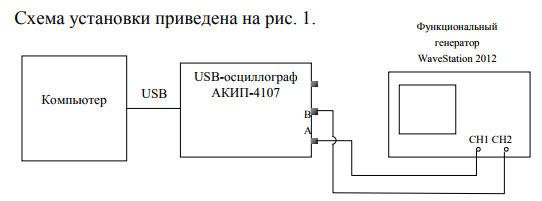
\includegraphics[width=0.6\linewidth]{1}
	\\
	\textbf{Рис.1} Экспериментальная установка
\end{figure}
\part*{Обработка результатов}
\part*{А. Исследование спектра периодической последовательности прямоугольных импульсов}
\textbf{1)} Начальные входные данные $V_0 = 1 $ В, $\tau = 100$ мкс, $f_{\text{повт}} = 1$ кГц.\\\\
При увеличении $\tau$ вдвое при неизменной частоте $f_{\text{повт}} = 1$ кГц $\delta \nu$ уменьшается вдвое. \\\\
При увеличении $f_{\text{повт}}$ вдвое при неизменной $\tau = 100$ мкс $\delta \nu$ увеличивается вдвое.
\newpage
\textbf{2)} Проведем измерения зависимости ширины спектра от длительности импульса $\Delta\nu(\tau)$:\\
\begin{table}[h!]
	\centering
	\textbf{Таблица 1}. Зависимость $\Delta\nu(\tau)$ \\
	\begin{tabular}{|r||c|c|c|c|c|c|c|c|c|c|c|}
		\hline 
		$\tau$,мкс & $40$ & $60$ & $80$ & $100$ & $120$ & $140$ & $160$ & $180$ & $200$ \\ 
		\hline
		$1/\tau,10^3 c^{-1}$ & $25,0$ & $16,7$ & $12,5$ & $10,0$ & $8,3$ & $7,1$ & $6,3$ & $5,6$ & $5,0$ \\ 
		\hline
		$\Delta\nu$,кГц & $25,0$ & $17,0$ & $12,5$ & $10,0$ & $7,5$ & $7,0$ & $6,0$ & $5,5$ & $5,0$ \\ 
		\hline
	\end{tabular}
\end{table}
\\
Построим график зависимости $\Delta\nu(\tau)$ и по его наклону убедимся в справедливости соотношения неопределённостей. \\
\begin{figure} [h!]
	\centering
		\textbf{График 1}. Зависимость $\Delta\nu(\tau)$ \\
	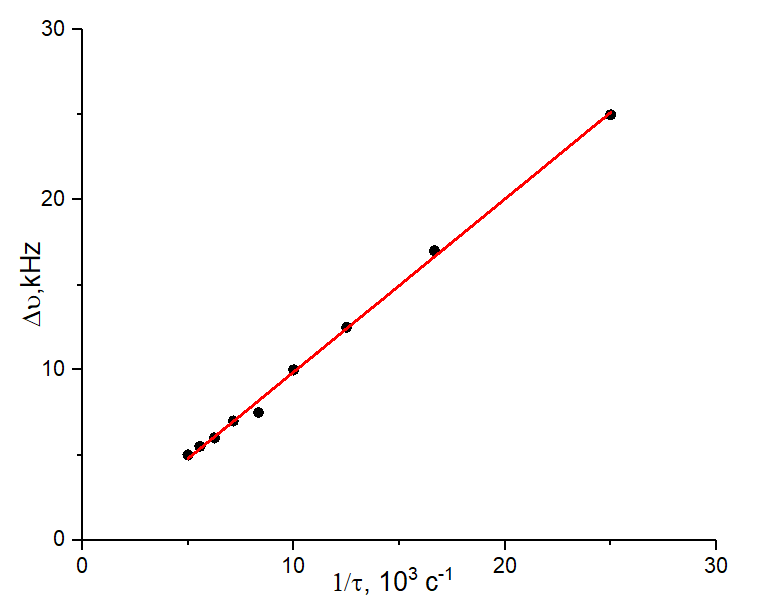
\includegraphics[width=0.7\linewidth]{2}
\end{figure}
\\
Тангенс наклона прямой, рассчитанный при помощи МНК, равен\\
$\boxed {k = 1,02 \pm 0,2 \ \  \text{Гц}\cdot c}.$\\\\что соответствует теоретическому значению.
\\
\\
\textbf{3)} Измерим частоты и амплитуды спектральных составляющих сигнала и запишем результаты в таблицы $2$ и $3$. 
	
	\begin{table} [h!]
		\centering
	\textbf{Таблица 2}. Частоты и амплитуды спектральных составляющих. \\
	$\tau = 50$ мкс.\\
\begin{tabular}{|r||c|c|c|c|c|c|c|c|c|c|c|c|}
	\hline 
	\textbf{№} & $\textbf{1}$ & $\textbf{2}$ & $\textbf{3}$ & $\textbf{4}$ & $\textbf{5}$ & $\textbf{6}$ & $\textbf{7}$ & $\textbf{8}$ & $\textbf{9}$ & $\textbf{10}$\\ 
	\hline
	\textbf {част, кГц} & $1,000$ & $2,000$ & $3,000$ & $4,000$ & $5,000$ & $6,000$ & $7,000$ & $8,000$ & $9,000$ & $ 10,000$ \\ 
	\hline
	\textbf {A, мВ} & $70,26$ & $69,32$ & $65,75$ & $63,05$ & $59,28$ & $57,72$ & $51,44$ & $47,99$ & $43,29$ & $40,78$ \\ 
	\hline
	\hline
	\textbf{№} & $\textbf{11}$ & $\textbf{12}$ & $\textbf{13}$ & $\textbf{14}$ & $\textbf{15}$ & $\textbf{16}$ & $\textbf{17}$ & $\textbf{18}$ & $\textbf{19}$ & $\textbf{20}$ \\ 
	\hline
	\textbf {част, кГц} & $11,000$ & $12,000$ & $13,000$ & $14,000$ & $15,000$ & $16,000$ & $17,000$ & $18,000$ & $19,000$ & $20,000$ \\ 
	\hline
	\textbf {A, мВ} & $37,01$ & $33,62$ & $29,77$ & $25,62$ & $21,38$ & $16,51$ & $12,45$ & $8,21$ & $3,61$ & $0,00$ \\ 
	\hline
\end{tabular}
\end{table}
\newpage
	\begin{table} [h!]
	\centering
	\textbf{Таблица 3}. Частоты и амплитуды спектральных составляющих. \\
	$\tau = 100$ мкс.\\
	\begin{tabular}{|r||c|c|c|c|c|c|c|c|c|c|c|c|}
		\hline 
		\textbf{№} & $\textbf{1}$ & $\textbf{2}$ & $\textbf{3}$ & $\textbf{4}$ & $\textbf{5}$ & $\textbf{6}$ & $\textbf{7}$ & $\textbf{8}$ & $\textbf{9}$ & $\textbf{10}$\\ 
		\hline
		\textbf {част, кГц} & $1,000$ & $2,000$ & $3,000$ & $4,000$ & $5,000$ & $6,000$ & $7,000$ & $8,000$ & $9,000$ & $ 10,000$ \\ 
		\hline
		\textbf {A, мВ} & $138,70$ & $131,10$ & $119,90$ & $103,40$ & $86,29$ & $66,78$ & $47,75$ & $29,52$ & $13,19$ & $1,26$ \\ 
		\hline
\end{tabular}
\end{table}
По полученным данным построим картины спектров (см. графики $2$ и $3$).
\part*{Б. Исследование спектра периодической последовательности цугов гармонических колебаний}
\textbf{4)}\\
Канал $1$: $V_0 = 1$ В, $f_{\text{повт}}=1$ кГц, $\tau=100$ мкс.\\
Канал $2$: $2A_{\text{сигн}} = 2$ В, $\nu_0 = 25$ кГц.\\\\
При увеличении длительности импульса $\tau$ вдвое $\delta \nu$ уменьшаться вдвое.\\\\
\textbf{5)} Установим частоту несущей $\nu_0 = 30$ кГц, длительность импульса $\tau = 100$ мкс. Проведём измерения расстояния $\delta \nu$ между соседними спектральными компонентами для разных частот $f_{\text{повт}}$.
\begin{table}[h!]
	\centering
	\textbf{Таблица 4}. Зависимость $\delta \nu (f_{\text{повт}})$ \\
	\begin{tabular}{|r||c|c|c|c|c|}
		\hline 
		$f_{pov}$,кГц & $0,5$ & $1,0$ & $2,0$ & $4,0$ & $5,0$ \\ 
		\hline
		$\delta\nu$,кГц & $0,5$ & $1,0$ & $2,0$ & $4,0$ & $5,0$ \\ 
		\hline
	\end{tabular}
\end{table}
\\
Построим график $\delta \nu (f_{\text{повт}})$.
\begin{figure} [h!]
	\centering
	\textbf{График 4} Зависимость $\delta \nu (f_{\text{повт}})$ \\
	\centering
	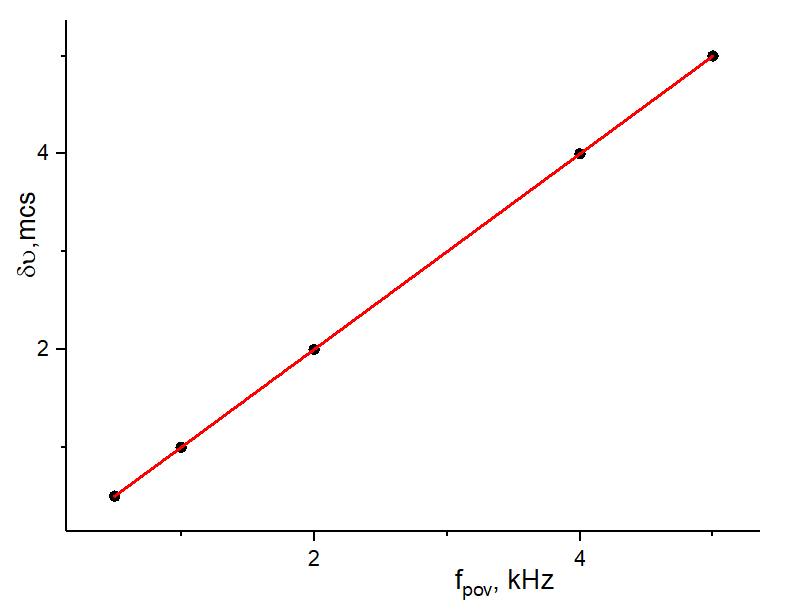
\includegraphics[width=0.6\linewidth]{3}
\end{figure}
\\
Тангенс наклона прямой $k=1$, что соответствует теоретическому значению.

\newpage

\textbf{6)} Установим $\tau = 100$ мкс, $f_{\text{повт}} = 1$ кГц. Определим амплитуды и частоты гармонического спектра. Проведём аналогичные измерения для $\tau = 100$ мкс и $f_{\text{повт}} = 2$ кГц. Данные занесём в таблицу $4$.
	\begin{table} [h!]
	\centering
	\textbf{Таблица 5}. Частоты и амплитуды спектральных составляющих.
	\begin{tabular}{|r||c|c|c|c|c|c|c|c|c|c|c|c|}
		\hline 
		\textbf{№} & $\textbf{1}$ & $\textbf{2}$ & $\textbf{3}$ & $\textbf{4}$ & $\textbf{5}$ & $\textbf{6}$ & $\textbf{7}$ & $\textbf{8}$ & $\textbf{9}$ & $\textbf{10}$\\ 
		\hline
		\textbf {$\nu_1$, кГц} & $31$ & $32$ & $33$ & $34$ & $35$ & $36$ & $37$ & $38$ & $39$ & $ 40$ \\ 
		\hline
		\textbf {$A_1$, мВ} & $1,831$ & $1,754$ & $1,626$ & $1,438$ & $1,136$ & $0,998$ & $0,626$ & $0,455$ & $0,223$ & $0,071$ \\ 
		\hline
		\hline
		\textbf{№} & $\textbf{1}$ & $\textbf{2}$ & $\textbf{3}$ & $\textbf{4}$ & $\textbf{5}$ & $\textbf{6}$ & $\textbf{7}$ & $\textbf{8}$ & $\textbf{9}$ & $\textbf{10}$ \\ 
		\hline
		\textbf {$\nu_2$, кГц} & $32$ & $34$ & $36$ & $38$ & $40$ & $42$ & $44$ & $46$ & $48$ & $50$ \\ 
		\hline
		\textbf {$A_2$, мВ} & $1,928$ & $1,677$ & $1,513$ & $1,271$ & $0,890$ & $0,734$ & $0,502$ & $0,346$ & $0,121$ & $0,034$ \\ 
		\hline
	\end{tabular}
\end{table}
\\
По полученным данным построим картины спектров (см. графики $5$ и $6$).\\\


\textbf{7)} Сравним построенные спектры:
\begin{enumerate}
	\item Прямоугольных импульсов при одинаковых $f_{\text{повт}}$ и разных $\tau$:\\
	$\delta \nu$ в $2$ раза больше у спектра $\tau = 50$ мкс
	\item Цугов при одинаковых $\tau$ и разных $f_{\text{повт}}$:\\
	$\delta \nu$ в $2$ раза больше у спектра $f_{\text{повт}} = 2$ кГц, чем $f_{\text{повт}} = 1$ кГц
	\item Цугов и прямоугольных импульсов при одинаковых $\tau$ и $f_{\text{повт}}$:\\
	спектры аналогичны, но максимум сдвинуты на $\nu_0$ вправо.	
\end{enumerate}
\part*{В. Исследование спектра гармноческих сигналов, модулированных по амплитуде}
\textbf{8)} \\
Канал $1$: смещение $1$ В, $f_{\text{мод}} = 1$ кГц, $2A = 0,2$ В.\\
Канал $2$: $2A=1$ В, смещение $0$ В, $\nu_0=25$ кГц \\\\
Меняя двойную амплитуду "CH1" от $0,2$В до 2В измерим для каждого значения $A_{max}$ и $A_{min}$ ампитудных сигналов и амплитуд спектральных компонент. Рассчитаем соответствущие значения глубины модуляции по формуле:\\
$m = \frac{A_{max}-A_{min}}{A_{max}+A_{min}}$
	\begin{table} [h!]
	\centering
	\textbf{Таблица 6}. Амплитуды сигнала и спектра.
	\begin{tabular}{|c|c|c|c|c|c|c|}
		\hline 
		$2A_{min}$,мВ & $2A_{max}$,мВ & $m$ & $a_{\text{осн}}$,кГц & $a_{\text{бок}}$,кГц & $a_{\text{осн}} / a_{\text{бок}}$ \\ \hline
		$114,6$ & $86,10$ & $0,14$ & $55,60$ & $2,899$ & $0,05$ \\ \hline
		$130,4$ & $74,29$ & $0,27$ & $55,28$ & $7,761$ & $0,14$ \\ \hline
		$143,2$ & $62,48$ & $0,39$ & $55,28$ & $11,840$ & $0,21$ \\ \hline
		$157,9$ & $45,76$ & $0,55$ & $55,44$ & $16,700$ & $0,30$ \\ \hline
		$173,7$ & $29,03$ & $0,71$ & $55,60$ & $20,460$ & $0,36$ \\ \hline
		$192,4$ & $15,25$ & $0,85$ & $55,60$ & $24,540$ & $0,44$ \\ \hline
		$200,5$ & $0,00$ & $1,00$ & $54,50$ & $29,720$ & $0,54$ \\ \hline
	\end{tabular}
\end{table}
\\
По полученным данным построим график зависимости $a_{\text{осн}} / a_{\text{бок}}$ от $m$.
\\
\begin{figure} [h!]
	\centering
	\textbf{График 7} Зависимость $a_{\text{осн}} / a_{\text{бок}}$ от $m$. \\
	\centering
	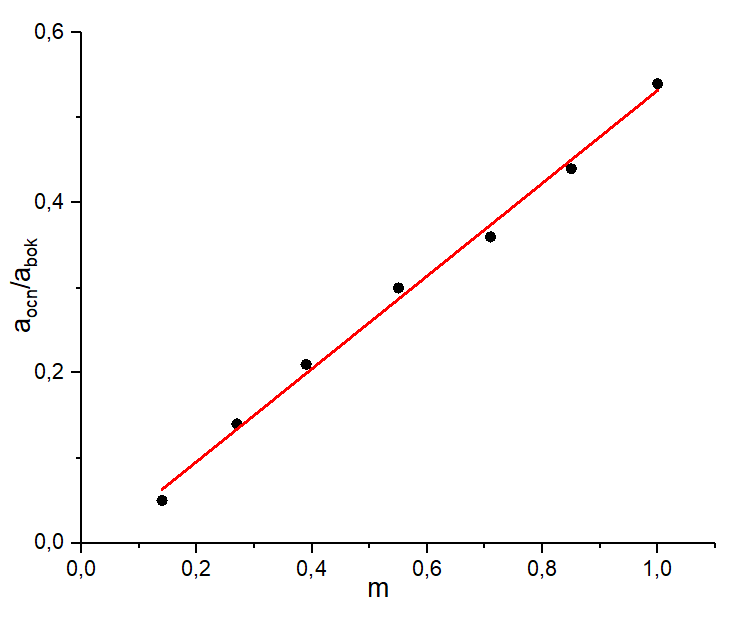
\includegraphics[width=0.55\linewidth]{4}
\end{figure}
\\
Найдём коэффициент наклона прямой при помощи МНК.
\\
$\boxed{k=0,55 \pm 0,01}$
\\\\
Теоретическое значение $k=0,5$
\\\\

\part*{Вывод}
\begin{enumerate}
	\item Экспериментально было проверено соотношение неопределённости в первых двух экспериментах. Полученные значения соответствуют ожидаемым.
	\item В третьем эксперименте была проверена зависимость амплитуд спектральных линий синусоидального сигнала, модулированного низкочастотными гармоническими колебаниями, от коэффициента модуляции.
\end{enumerate}
\end{document}